\documentclass{standalone}
\usepackage{tikz, xcolor}
\usetikzlibrary{shapes,arrows}

\begin{document}

\begin{tikzpicture}[thick, scale=2.0]
\tikzstyle{vertexr}=[rectangle, draw=blue, thick, minimum size=14pt, inner sep=2pt]
\tikzstyle{vertexc}=[circle, draw=blue, thick, inner sep=2pt]
\tikzstyle{drawstyle}=[thick, ->]

\node[vertexr] (G0x0) at (0,0) {int gx};
\node[vertexr] (G1x0) at (1,0) {int gy};
\node[vertexr] (G2x0) at (2,0) {void Func fred};
\node[vertexr] (G2x1) at (2,-1) {int px};
\node[vertexr] (G3x1) at (3,-1) {int py};
\draw[drawstyle] (G2x1) -- (G3x1);
\draw[drawstyle] (G2x0) -- (G2x1);
\node[vertexr] (G4x1) at (4,-1) {Compound};
\node[vertexr] (G4x2) at (4,-2) {int x};
\node[vertexr] (G5x2) at (5,-2) {int y};
\node[vertexr] (G6x2) at (6,-2) {int sx};
\node[vertexr] (G7x2) at (7,-2) {int sy};
\draw[drawstyle] (G6x2) -- (G7x2);
\draw[drawstyle] (G5x2) -- (G6x2);
\draw[drawstyle] (G4x2) -- (G5x2);
\draw[drawstyle] (G4x1) -- (G4x2);
\node[vertexr] (G8x2) at (8,-2) {=};
\node[vertexr] (G8x3) at (8,-3) {gx};
\draw[drawstyle] (G8x2) -- (G8x3);
\node[vertexr] (G9x3) at (9,-3) {111};
\draw[drawstyle] (G8x2) -- (G9x3);
\node[vertexr] (G10x2) at (10,-2) {=};
\node[vertexr] (G10x3) at (10,-3) {gx};
\draw[drawstyle] (G10x2) -- (G10x3);
\node[vertexr] (G11x3) at (11,-3) {gx};
\draw[drawstyle] (G10x2) -- (G11x3);
\node[vertexr] (G12x2) at (12,-2) {Call output};
\node[vertexr] (G12x3) at (12,-3) {gx};
\draw[drawstyle] (G12x2) -- (G12x3);
\node[vertexr] (G13x2) at (13,-2) {=};
\node[vertexr] (G13x3) at (13,-3) {gy};
\node[vertexr] (G13x4) at (13,-4) {9};
\draw[drawstyle] (G13x3) -- (G13x4);
\draw[drawstyle] (G13x2) -- (G13x3);
\node[vertexr] (G14x3) at (14,-3) {222};
\draw[drawstyle] (G13x2) -- (G14x3);
\node[vertexr] (G15x2) at (15,-2) {=};
\node[vertexr] (G15x3) at (15,-3) {gy};
\node[vertexr] (G15x4) at (15,-4) {9};
\draw[drawstyle] (G15x3) -- (G15x4);
\draw[drawstyle] (G15x2) -- (G15x3);
\node[vertexr] (G16x3) at (16,-3) {gy};
\node[vertexr] (G16x4) at (16,-4) {9};
\draw[drawstyle] (G16x3) -- (G16x4);
\draw[drawstyle] (G15x2) -- (G16x3);
\node[vertexr] (G17x2) at (17,-2) {Call output};
\node[vertexr] (G17x3) at (17,-3) {gy};
\node[vertexr] (G17x4) at (17,-4) {9};
\draw[drawstyle] (G17x3) -- (G17x4);
\draw[drawstyle] (G17x2) -- (G17x3);
\node[vertexr] (G18x2) at (18,-2) {Call outnl};
\node[vertexr] (G19x2) at (19,-2) {=};
\node[vertexr] (G19x3) at (19,-3) {x};
\draw[drawstyle] (G19x2) -- (G19x3);
\node[vertexr] (G20x3) at (20,-3) {333};
\draw[drawstyle] (G19x2) -- (G20x3);
\node[vertexr] (G21x2) at (21,-2) {=};
\node[vertexr] (G21x3) at (21,-3) {x};
\draw[drawstyle] (G21x2) -- (G21x3);
\node[vertexr] (G22x3) at (22,-3) {x};
\draw[drawstyle] (G21x2) -- (G22x3);
\node[vertexr] (G23x2) at (23,-2) {Call output};
\node[vertexr] (G23x3) at (23,-3) {x};
\draw[drawstyle] (G23x2) -- (G23x3);
\node[vertexr] (G24x2) at (24,-2) {=};
\node[vertexr] (G24x3) at (24,-3) {y};
\node[vertexr] (G24x4) at (24,-4) {9};
\draw[drawstyle] (G24x3) -- (G24x4);
\draw[drawstyle] (G24x2) -- (G24x3);
\node[vertexr] (G25x3) at (25,-3) {444};
\draw[drawstyle] (G24x2) -- (G25x3);
\node[vertexr] (G26x2) at (26,-2) {=};
\node[vertexr] (G26x3) at (26,-3) {y};
\node[vertexr] (G26x4) at (26,-4) {9};
\draw[drawstyle] (G26x3) -- (G26x4);
\draw[drawstyle] (G26x2) -- (G26x3);
\node[vertexr] (G27x3) at (27,-3) {y};
\node[vertexr] (G27x4) at (27,-4) {9};
\draw[drawstyle] (G27x3) -- (G27x4);
\draw[drawstyle] (G26x2) -- (G27x3);
\node[vertexr] (G28x2) at (28,-2) {Call output};
\node[vertexr] (G28x3) at (28,-3) {y};
\node[vertexr] (G28x4) at (28,-4) {9};
\draw[drawstyle] (G28x3) -- (G28x4);
\draw[drawstyle] (G28x2) -- (G28x3);
\node[vertexr] (G29x2) at (29,-2) {Call outnl};
\node[vertexr] (G30x2) at (30,-2) {=};
\node[vertexr] (G30x3) at (30,-3) {px};
\draw[drawstyle] (G30x2) -- (G30x3);
\node[vertexr] (G31x3) at (31,-3) {555};
\draw[drawstyle] (G30x2) -- (G31x3);
\node[vertexr] (G32x2) at (32,-2) {=};
\node[vertexr] (G32x3) at (32,-3) {px};
\draw[drawstyle] (G32x2) -- (G32x3);
\node[vertexr] (G33x3) at (33,-3) {px};
\draw[drawstyle] (G32x2) -- (G33x3);
\node[vertexr] (G34x2) at (34,-2) {Call output};
\node[vertexr] (G34x3) at (34,-3) {px};
\draw[drawstyle] (G34x2) -- (G34x3);
\node[vertexr] (G35x2) at (35,-2) {=};
\node[vertexr] (G35x3) at (35,-3) {py};
\node[vertexr] (G35x4) at (35,-4) {9};
\draw[drawstyle] (G35x3) -- (G35x4);
\draw[drawstyle] (G35x2) -- (G35x3);
\node[vertexr] (G36x3) at (36,-3) {666};
\draw[drawstyle] (G35x2) -- (G36x3);
\node[vertexr] (G37x2) at (37,-2) {=};
\node[vertexr] (G37x3) at (37,-3) {py};
\node[vertexr] (G37x4) at (37,-4) {9};
\draw[drawstyle] (G37x3) -- (G37x4);
\draw[drawstyle] (G37x2) -- (G37x3);
\node[vertexr] (G38x3) at (38,-3) {py};
\node[vertexr] (G38x4) at (38,-4) {9};
\draw[drawstyle] (G38x3) -- (G38x4);
\draw[drawstyle] (G37x2) -- (G38x3);
\node[vertexr] (G39x2) at (39,-2) {Call output};
\node[vertexr] (G39x3) at (39,-3) {py};
\node[vertexr] (G39x4) at (39,-4) {9};
\draw[drawstyle] (G39x3) -- (G39x4);
\draw[drawstyle] (G39x2) -- (G39x3);
\node[vertexr] (G40x2) at (40,-2) {Call outnl};
\node[vertexr] (G41x2) at (41,-2) {=};
\node[vertexr] (G41x3) at (41,-3) {sx};
\draw[drawstyle] (G41x2) -- (G41x3);
\node[vertexr] (G42x3) at (42,-3) {777};
\draw[drawstyle] (G41x2) -- (G42x3);
\node[vertexr] (G43x2) at (43,-2) {=};
\node[vertexr] (G43x3) at (43,-3) {sx};
\draw[drawstyle] (G43x2) -- (G43x3);
\node[vertexr] (G44x3) at (44,-3) {sx};
\draw[drawstyle] (G43x2) -- (G44x3);
\node[vertexr] (G45x2) at (45,-2) {Call output};
\node[vertexr] (G45x3) at (45,-3) {sx};
\draw[drawstyle] (G45x2) -- (G45x3);
\node[vertexr] (G46x2) at (46,-2) {=};
\node[vertexr] (G46x3) at (46,-3) {sy};
\node[vertexr] (G46x4) at (46,-4) {9};
\draw[drawstyle] (G46x3) -- (G46x4);
\draw[drawstyle] (G46x2) -- (G46x3);
\node[vertexr] (G47x3) at (47,-3) {888};
\draw[drawstyle] (G46x2) -- (G47x3);
\node[vertexr] (G48x2) at (48,-2) {=};
\node[vertexr] (G48x3) at (48,-3) {sy};
\node[vertexr] (G48x4) at (48,-4) {9};
\draw[drawstyle] (G48x3) -- (G48x4);
\draw[drawstyle] (G48x2) -- (G48x3);
\node[vertexr] (G49x3) at (49,-3) {sy};
\node[vertexr] (G49x4) at (49,-4) {9};
\draw[drawstyle] (G49x3) -- (G49x4);
\draw[drawstyle] (G48x2) -- (G49x3);
\node[vertexr] (G50x2) at (50,-2) {Call output};
\node[vertexr] (G50x3) at (50,-3) {sy};
\node[vertexr] (G50x4) at (50,-4) {9};
\draw[drawstyle] (G50x3) -- (G50x4);
\draw[drawstyle] (G50x2) -- (G50x3);
\node[vertexr] (G51x2) at (51,-2) {Call outnl};
\draw[drawstyle] (G50x2) -- (G51x2);
\draw[drawstyle] (G48x2) -- (G50x2);
\draw[drawstyle] (G46x2) -- (G48x2);
\draw[drawstyle] (G45x2) -- (G46x2);
\draw[drawstyle] (G43x2) -- (G45x2);
\draw[drawstyle] (G41x2) -- (G43x2);
\draw[drawstyle] (G40x2) -- (G41x2);
\draw[drawstyle] (G39x2) -- (G40x2);
\draw[drawstyle] (G37x2) -- (G39x2);
\draw[drawstyle] (G35x2) -- (G37x2);
\draw[drawstyle] (G34x2) -- (G35x2);
\draw[drawstyle] (G32x2) -- (G34x2);
\draw[drawstyle] (G30x2) -- (G32x2);
\draw[drawstyle] (G29x2) -- (G30x2);
\draw[drawstyle] (G28x2) -- (G29x2);
\draw[drawstyle] (G26x2) -- (G28x2);
\draw[drawstyle] (G24x2) -- (G26x2);
\draw[drawstyle] (G23x2) -- (G24x2);
\draw[drawstyle] (G21x2) -- (G23x2);
\draw[drawstyle] (G19x2) -- (G21x2);
\draw[drawstyle] (G18x2) -- (G19x2);
\draw[drawstyle] (G17x2) -- (G18x2);
\draw[drawstyle] (G15x2) -- (G17x2);
\draw[drawstyle] (G13x2) -- (G15x2);
\draw[drawstyle] (G12x2) -- (G13x2);
\draw[drawstyle] (G10x2) -- (G12x2);
\draw[drawstyle] (G8x2) -- (G10x2);
\draw[drawstyle] (G4x1) -- (G8x2);
\draw[drawstyle] (G2x0) -- (G4x1);
\node[vertexr] (G52x0) at (52,0) {void Func main};
\node[vertexc] (G52x1) at (52,-1) {.};
\draw[drawstyle] (G52x0) -- (G52x1);
\node[vertexr] (G53x1) at (53,-1) {Compound};
\node[vertexr] (G53x2) at (53,-2) {int lx};
\node[vertexr] (G54x2) at (54,-2) {int ly};
\draw[drawstyle] (G53x2) -- (G54x2);
\draw[drawstyle] (G53x1) -- (G53x2);
\node[vertexr] (G55x2) at (55,-2) {Call fred};
\node[vertexr] (G55x3) at (55,-3) {gx};
\node[vertexr] (G56x3) at (56,-3) {gy};
\draw[drawstyle] (G55x3) -- (G56x3);
\draw[drawstyle] (G55x2) -- (G55x3);
\node[vertexr] (G57x2) at (57,-2) {Call fred};
\node[vertexr] (G57x3) at (57,-3) {lx};
\node[vertexr] (G58x3) at (58,-3) {ly};
\draw[drawstyle] (G57x3) -- (G58x3);
\draw[drawstyle] (G57x2) -- (G57x3);
\draw[drawstyle] (G55x2) -- (G57x2);
\draw[drawstyle] (G53x1) -- (G55x2);
\draw[drawstyle] (G52x0) -- (G53x1);
\draw[drawstyle] (G2x0) -- (G52x0);
\draw[drawstyle] (G1x0) -- (G2x0);
\draw[drawstyle] (G0x0) -- (G1x0);
\end{tikzpicture}
\end{document}
Number of warnings: 0
Number of errors: 0
